% Supplementary / Extended Data Figures for Zutshi et al. 2025
% Chapter: Hippocampal neuronal activity is aligned with action plans

\section*{Extended Data Figures}

\begin{figure}[htbp]
\centering

\includegraphics[width=\textwidth]{figures/ch_zutshi2025/extended_fig1.jpg}
\caption[Extended Data Fig.~1: Behavioral variability for ports 1--6]{\textbf{Extended Data Fig.~1: Behavioral variability for ports 1--6.}
(a) Spectrogram of frequencies recorded in an incorrect and correct trial, with error tone (3\,kHz, 1\,s) and water delivery shown.
(b) Probability of trials was unevenly distributed to yield more trials where mice performed close to the target port.
(c--e) Tone frequency progression separated by errors one, two, or three ports before the target.
(f) Histogram of difference between the choice and target port for regular (grey) and probe (purple) trials; 4-kHz trials showed undershooting errors, 8-kHz trials showed both undershooting and overshooting.
(g--h) Behavioral performance during probe trials by port and by probe frequency.}
\label{fig:zutshi2025-ext1}
\end{figure}

\begin{figure}[htbp]
\centering

\includegraphics[width=\textwidth]{figures/ch_zutshi2025/extended_fig2.jpg}
\caption[Extended Data Fig.~2: Modulation of hippocampal cells by space and approach to ports]{\textbf{Extended Data Fig.~2: Modulation of hippocampal cells by space and approach to ports.}
(a) Additional examples of CA1 pyramidal cell firing with place, mixed, and tone tuning.
(b--c) Fraction and number of active pyramidal cells responding to the tone per session.
(d--e) Proportion of tone cells with stable place fields during no-tone trials.
(f--h) During error trials, tone cell firing reflected the approach to the chosen port rather than the target port ($n=1129$ cells from 37 sessions in 6 mice; Wilcoxon two-sided paired signed-rank test, $z=-18.96$, $p=3.47\times10^{-80}$).
(i) All cells with a significant firing field during tone trials ordered by spatial preference; spatial tuning persisted but was significantly altered between NT1 and tone trials.
(j--k) Six example cells showing spatial field shifts with varying run lengths during tone trials.}
\label{fig:zutshi2025-ext2}
\end{figure}

\begin{figure}[htbp]
\centering

\includegraphics[width=\textwidth]{figures/ch_zutshi2025/extended_fig3.jpg}
\caption[Extended Data Fig.~3: Fitting multiple behavior variables to model single-cell firing]{\textbf{Extended Data Fig.~3: Fitting multiple behavior variables to model single-cell firing.}
(a) Schematic of the Poisson generalized additive model (P-GAM) with continuous task variables (position in NT and tone trials, progression-to-choice) and discrete lick events as inputs.
(b--h) P-GAM fit quality, mutual information distributions, and tuning comparisons across variables.
(i) Distribution of the ratio of MI for position versus progression-to-choice for dually modulated cells ($n=1197$ cells tuned to position, 189 cells tuned to progression-to-choice).
(j) Scatter of kernel strength of choice licks during tone trials versus spontaneous licks, confirming co-modulation.}
\label{fig:zutshi2025-ext3}
\end{figure}

\begin{figure}[htbp]
\centering

\includegraphics[width=\textwidth]{figures/ch_zutshi2025/extended_fig4.jpg}
\caption[Extended Data Fig.~4: Phase precession of place and tone cells by approach to each port]{\textbf{Extended Data Fig.~4: Phase precession of place and tone cells by approach to each port.}
(a) Five example cells (3 place cells, 2 tone cells) showing average rate maps and theta-phase by position plots for each port approach.
(b--c) Average phase precession slopes and intercepts of place cells with significant slopes across port approaches ($n=80$--344 cells; Kruskal--Wallis test: slope $\chi^2(4,3097)=1.42$, $p=0.84$; intercept $\chi^2(4,3097)=0.55$, $p=0.97$).
(d) Average phase precession slopes and intercepts of place cells with significant slopes ($n=80$--344 cells; slope $\chi^2(4,1048)=10.69$, $p=0.03$; intercept $\chi^2(4,1048)=1.56$, $p=0.82$).}
\label{fig:zutshi2025-ext4}
\end{figure}

\begin{figure}[htbp]
\centering

\includegraphics[width=\textwidth]{figures/ch_zutshi2025/extended_fig5.jpg}
\caption[Extended Data Fig.~5: Theta sequences observed for both place and tone cells]{\textbf{Extended Data Fig.~5: Theta sequences observed for both place and tone cells.}
(a) Spike rasters from an example session sorted using Rastermap; black dots = place cells, pink dots = tone cells, grey dots = non-classified cells. Blue trace: LFP filtered in the theta band (6--12\,Hz). Place cell sequences precede tone cell firing in the 0.5\,s preceding the lick.
(b--c) Example cross-correlograms (CCG) between a place cell pair (b) and a tone cell pair (c), showing theta-band coordination.
(d) Distance-to-time compression for place cell pairs (top) and tone cell pairs (bottom).}
\label{fig:zutshi2025-ext5}
\end{figure}

\begin{figure}[htbp]
\centering

\includegraphics[width=\textwidth]{figures/ch_zutshi2025/extended_fig6.jpg}
\caption[Extended Data Fig.~6: Evolution of cell assemblies and controls for spatial remapping]{\textbf{Extended Data Fig.~6: Evolution of cell assemblies and controls for spatial remapping.}
(a) Cell assembly activation across all sessions, sorted by activation profile and separated by ports 1--6; temporal width of the sequence expands from ports 1 to 6.
(b--g) Quantification of assembly sequences, peak latencies, and their relationship to spatial remapping.
(h--k) Control task: trajectory, lick heatmap, and example CA1 pyramidal cell from a mouse trained with no tone-significance (reward fixed at end port). No remapping was observed between NT1 and tone trials in control mice.}
\label{fig:zutshi2025-ext6}
\end{figure}

\begin{figure}[htbp]
\centering

\includegraphics[width=\textwidth]{figures/ch_zutshi2025/extended_fig7.jpg}
\caption[Extended Data Fig.~7: Spatial remapping depends on the mouse's running trajectory]{\textbf{Extended Data Fig.~7: Spatial remapping depends on the mouse's running trajectory.}
(a) Movement trajectory (mean $\pm$ s.e.m.) across all mice for NT1, tone port 6, and NT2 trials; mice avoided the port wall in NT1, ran along the port wall in tone trials, and midway during NT2.
(b) Average standard deviation of the trajectory by trial type.
(c--e) Rate map correlations within and across conditions for cells with matched versus different trajectories.
(f) Spikes from an example cell overlaid with trajectories clustered by distance from the top wall; rate maps computed separately for each cluster.}
\label{fig:zutshi2025-ext7}
\end{figure}

\begin{figure}[htbp]
\centering

\includegraphics[width=\textwidth]{figures/ch_zutshi2025/extended_fig8.jpg}
\caption[Extended Data Fig.~8: Similar evolution of cell assemblies during non-probe and probe trials]{\textbf{Extended Data Fig.~8: Similar evolution of cell assemblies during non-probe and probe trials.}
(a) Spatial maps of tone cells during non-probe and probe trials (sorted as Fig.~3b); probe trials restricted to ports 3--6.
(b) Rate maps of two example place fields separated by port trajectory for probe and non-probe trials.
(c) Firing rate maps of all place cells detected using tone port 6 trials.
(d--f) Assembly sequences sorted by latency in non-probe trials and maintained for probe trials; a stable cell assembly sequence persisted during probe trials, particularly in the $\sim$1\,s preceding the lick.
(g) Spike rasters (rastermap-sorted) for one non-probe, one probe-correct, and one probe-incorrect trial.}
\label{fig:zutshi2025-ext8}
\end{figure}

\begin{figure}[htbp]
\centering

\includegraphics[width=\textwidth]{figures/ch_zutshi2025/extended_fig9.jpg}
\caption[Extended Data Fig.~9: Tone cells were not directly modulated by reward or running speed]{\textbf{Extended Data Fig.~9: Tone cells were not directly modulated by reward or running speed.}
(a) PSTH of tone cells for choice licks during tone trials, separated by correct (rewarded) and incorrect (unrewarded) licks; no significant difference observed.
(b--f) Speed analysis and additional lick-type comparisons confirming that firing was not a uniform reward-expectation signal.
(g) Average PSTH of reward-related tone cells for choice licks during tone trials separated by port number; later (higher-probability) ports had lower firing rate modulation ($n=633$ cells from 6 mice; Friedman test, $\chi^2(5,3160)=77.96$, $p=2.24\times10^{-15}$).}
\label{fig:zutshi2025-ext9}
\end{figure}

\begin{figure}[htbp]
\centering

\includegraphics[width=\textwidth]{figures/ch_zutshi2025/extended_fig10.jpg}
\caption[Extended Data Fig.~10: Firing rate maps do not change or overrepresent a new reward]{\textbf{Extended Data Fig.~10: Firing rate maps do not change or overrepresent a new reward.}
(a) Example trajectories highlighting behavioral differences after the change in reward condition; mice often ran incomplete trajectories to the unrewarded port in the 1-port condition.
(b) Trial block correlation for two example CA1 pyramidal cells across the reward condition change.
(c) Distribution of place field peak locations for forward and reverse runs.
(d--e) Selection criteria for cells used in the correlation analysis.
(f) Average cell-by-cell trial block correlation for selected neurons; condition change between trial blocks 5 and 6.
(g) Average cell-by-cell correlation between blocks 3--4, 5--6, and 7--8 for each running direction (Friedman test; $n=39$ forward-run place cells, $\chi^2(2,37)=2.00$, $p=0.37$; $n=61$ return-run place cells).}
\label{fig:zutshi2025-ext10}
\end{figure}

\begin{figure}[htbp]
\centering
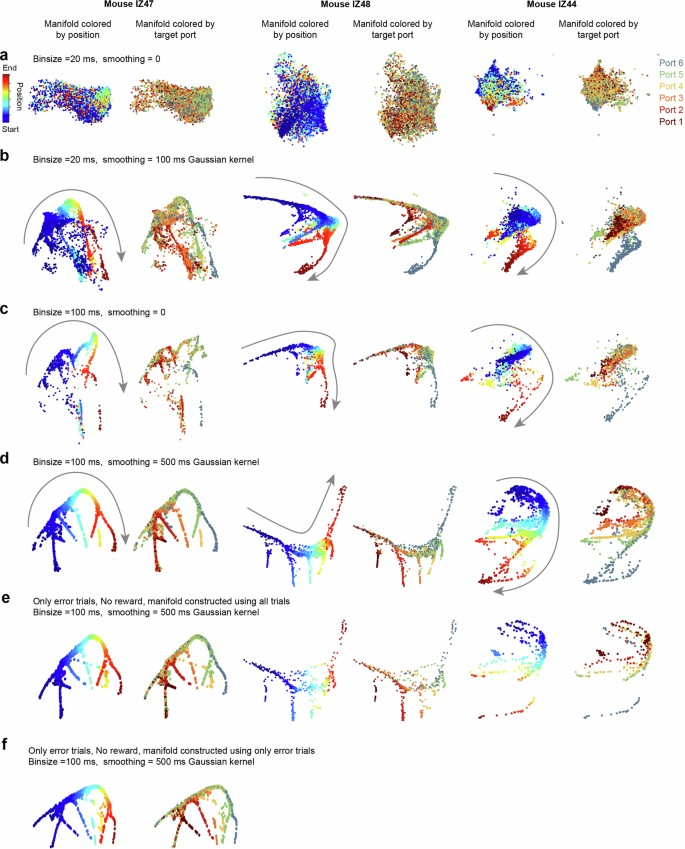
\includegraphics[width=\textwidth]{figures/ch_zutshi2025/extended_fig11.jpg}
\caption[Extended Data Fig.~11: Effect of binning, smoothing, and rewards on the neural manifold]{\textbf{Extended Data Fig.~11: Effect of binning, smoothing, and rewards on the neural manifold.}
Neural manifolds from three example sessions (mice IZ47, IZ48, IZ44) with varying time bin widths and Gaussian smoothing kernels. The 100-ms bin / 500-ms smoothing condition produced the most consistent manifold shape across sessions. Branches were also observed with lower binning and smoothing. Error trial manifold was also preserved, suggesting reward has no major role in the manifold structure.}
\label{fig:zutshi2025-ext11}
\end{figure}

\begin{figure}[htbp]
\centering
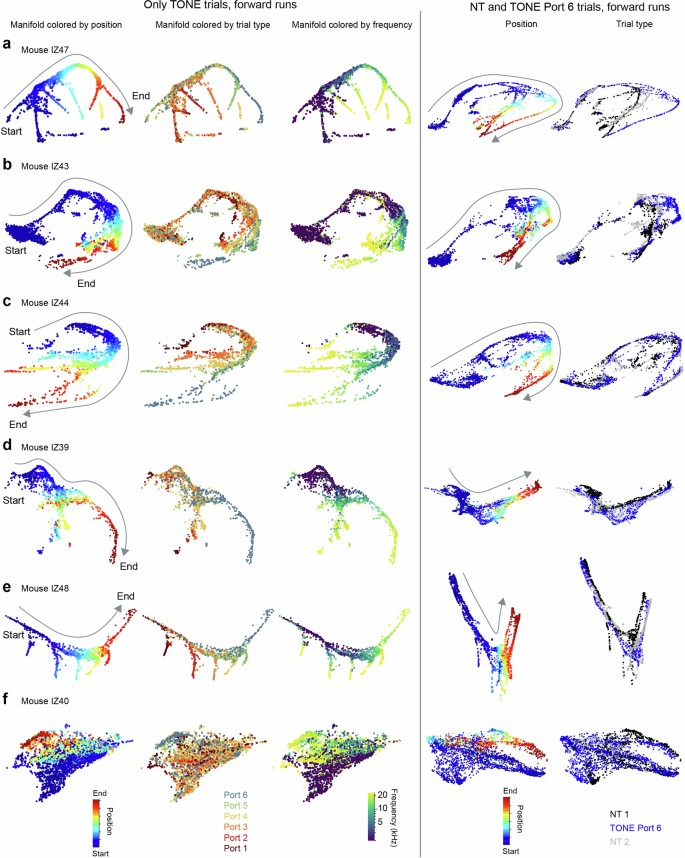
\includegraphics[width=\textwidth]{figures/ch_zutshi2025/extended_fig12.jpg}
\caption[Extended Data Fig.~12: Distinct branches in the neural manifold observed across several mice]{\textbf{Extended Data Fig.~12: Distinct branches in the neural manifold observed across several mice.}
(a--f) Neural manifolds from example sessions from six mice, coloured by spatial position, target port, and auditory frequency. Neural trajectories diverged into port-specific branches at approximately 8--10\,kHz, consistent across animals. NT1 and tone trial manifolds also shown; trajectories differed by trial type, with port 6 tone and NT2 trials yielding more similar trajectories.}
\label{fig:zutshi2025-ext12}
\end{figure}

\begin{figure}[htbp]
\centering
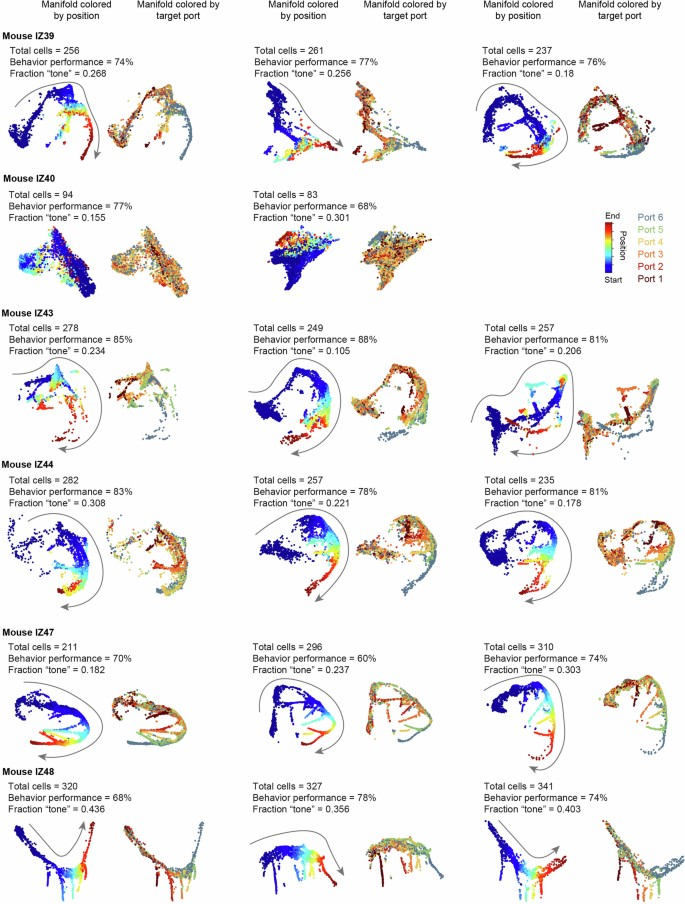
\includegraphics[width=\textwidth]{figures/ch_zutshi2025/extended_fig13.jpg}
\caption[Extended Data Fig.~13: Variability in the neural manifold across sessions and animals]{\textbf{Extended Data Fig.~13: Variability in the neural manifold across sessions and animals.}
UMAP displays of 2--3 sessions (columns) from each animal (rows), showing only forward runs of correct tone trials, coloured by spatial position (left) and chosen port (right). The total number of recorded cells, behavioral performance, and fraction of tone cells are indicated per session. Remarkable consistency was observed across sessions within the same animal, with similar features preserved across animals.}
\label{fig:zutshi2025-ext13}
\end{figure}

\begin{figure}[htbp]
\centering
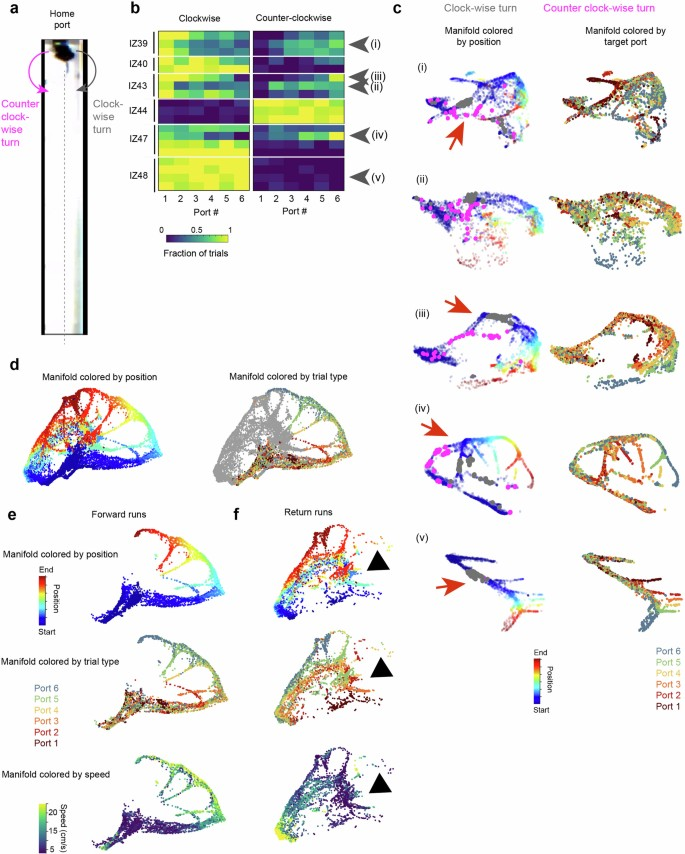
\includegraphics[width=\textwidth]{figures/ch_zutshi2025/extended_fig14.jpg}
\caption[Extended Data Fig.~14: Direction of rotation and movement is reflected in the neural manifold]{\textbf{Extended Data Fig.~14: Direction of rotation and movement is reflected in the neural manifold.}
(a) Top-view schematic of the mouse at the home port, showing clockwise (grey) and counter-clockwise (pink) turn options.
(b) Fraction of clockwise versus counter-clockwise turns by session and animal; some mice strongly preferred one direction, others showed port-dependent preferences.
(c) Neural manifold coloured by position and turn direction.
(d--e) Complete neural manifold including forward and return runs, showing forward run branches for each target port.
(f) Return run time points from the same manifold.}
\label{fig:zutshi2025-ext14}
\end{figure}

\begin{figure}[htbp]
\centering
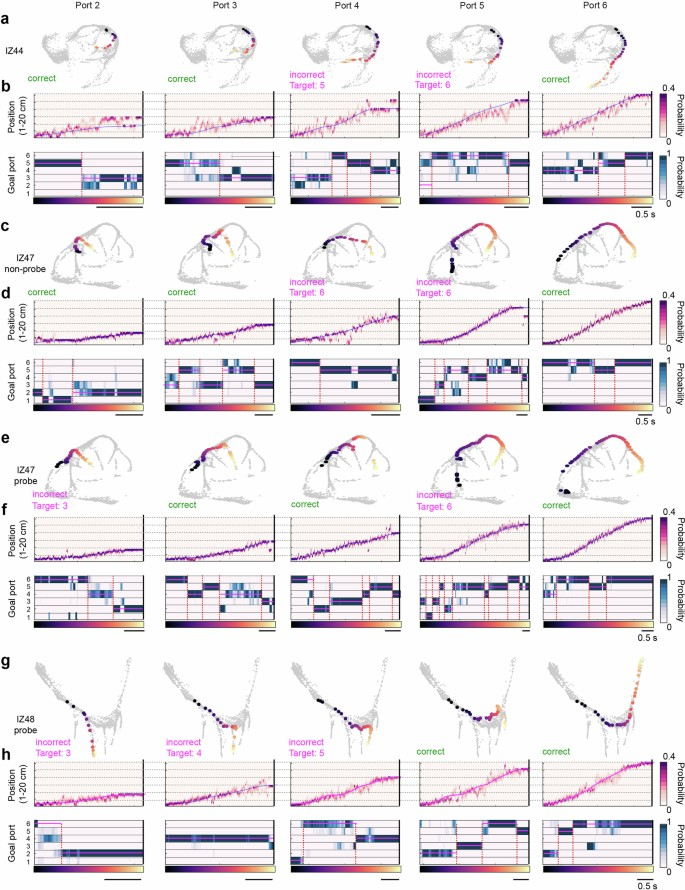
\includegraphics[width=\textwidth]{figures/ch_zutshi2025/extended_fig15.jpg}
\caption[Extended Data Fig.~15: Examples of single-trial UMAP displays and position/goal decoding across mice]{\textbf{Extended Data Fig.~15: Examples of single-trial UMAP displays and position/goal decoding across mice.}
(a--b) UMAP overlaid with single trials going to target ports 2--6 (mouse IZ44), with 2D spatial position and goal decoding shown in 10-ms time bins.
(c--d) Same for non-probe trials from mouse IZ47.
(e--f) Same for 4-kHz probe trials from the same session; neural manifold trajectory, goal, and position decoding evolved similarly to non-probe trials.
(g--h) Probe trials from mouse IZ48, demonstrating consistency across animals.}
\label{fig:zutshi2025-ext15}
\end{figure}

\begin{figure}[htbp]
\centering
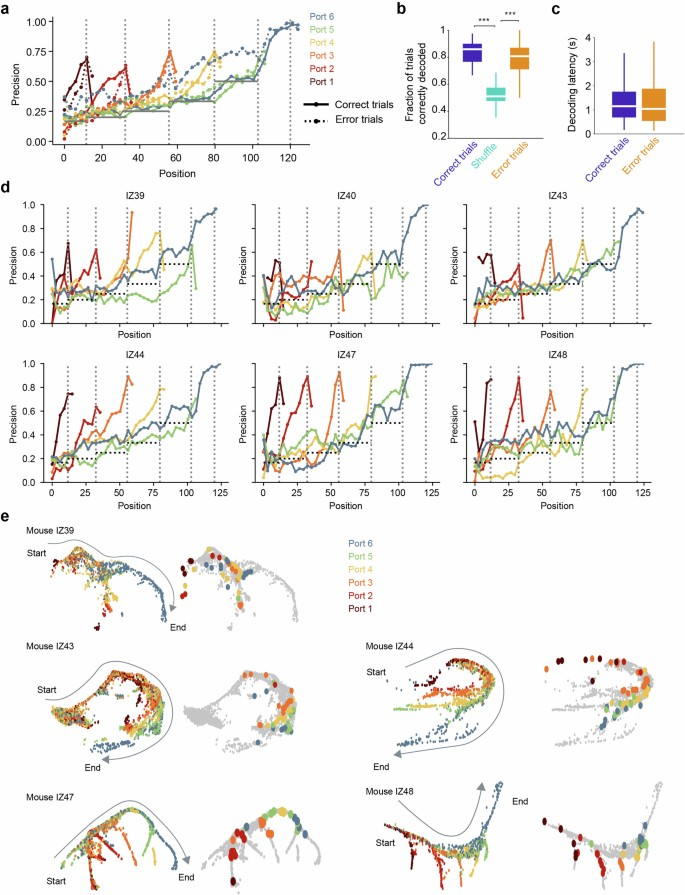
\includegraphics[width=\textwidth]{figures/ch_zutshi2025/extended_fig16.jpg}
\caption[Extended Data Fig.~16: The target goal can be predicted from population activity]{\textbf{Extended Data Fig.~16: The target goal can be predicted from population activity.}
(a) Goal port decoding from population spiking as a function of position; the decoder predicted the target port above chance before the mouse reached the chosen port (37 sessions in 6 mice).
(b) Final decoded goal compared to the mouse's choice using the change-point method; both correct and error trials predicted.
(c) Time before the lick when the target port could be correctly predicted in correct and error trials (${\sim}1.1$\,s; $n=1644, 519$ trials; Wilcoxon two-sided rank-sum test, $z=0.9$, $p=0.37$).
(d) Same as (a) for individual animals; mouse IZ40 with few cells showed poor decoding performance.
(e) Example neural manifold for each animal (except IZ40) coloured by target port (left) and with change-point timestamps superimposed (right).}
\label{fig:zutshi2025-ext16}
\end{figure}

\begin{figure}[htbp]
\centering
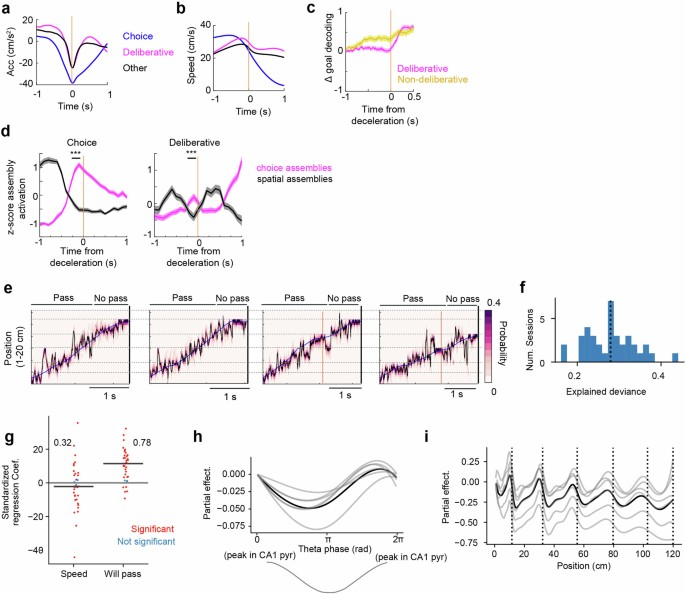
\includegraphics[width=\textwidth]{figures/ch_zutshi2025/extended_fig17.jpg}
\caption[Extended Data Fig.~17: Relationship between speed deceleration and theta look-ahead within a trial]{\textbf{Extended Data Fig.~17: Relationship between speed deceleration and theta look-ahead within a trial.}
(a) All significant decelerations during forward tone trials categorised as choice (blue), deliberative (pink), and other (black); choice decelerations had more pronounced troughs.
(b) Speed profiles for each deceleration category; despite significant deceleration, speed remained high during deliberative events.
(c) Change in goal decoding from the neuronal population against deliberative decelerations; yellow control extracted from random port-crossing times without deceleration.
(d) Expression of choice (pink) and spatial (black) cell assemblies during deceleration events; choice assemblies transiently increased while spatial assemblies decreased during deliberative decelerations ($n=90$ choice, 59 spatial assemblies; Wilcoxon rank-sum test, choice: $p=5.89\times10^{-13}$, deliberation: $p=1.62\times10^{-4}$).
(e) Four example trials showing position decoding, with higher likelihood of decoding beyond the next port if the mouse will pass versus lick.
(f--i) GAM fit predicting position decoding posterior beyond the upcoming port using speed, will\_pass, theta phase, and position regressors; the ascending phase of theta showed greater look-ahead.}
\label{fig:zutshi2025-ext17}
\end{figure}
